Esta captura se realizó a partir de una red doméstica, con dos computadoras conectadas por cable ethernet y varios dispositivos wireless (celulares, impresora y chromecast).

\textbf{Fuente S}:
La entropía obtenida (aproximadamente 0.924) se acerca bastante a la máxima, a diferencia de las otras capturas que poseen una entropía muy baja. Además como se observa en el gráfico, la proporción de mensajes unicast fue mayor que la de broadcast.	

\begin{figure}[h]
\centering
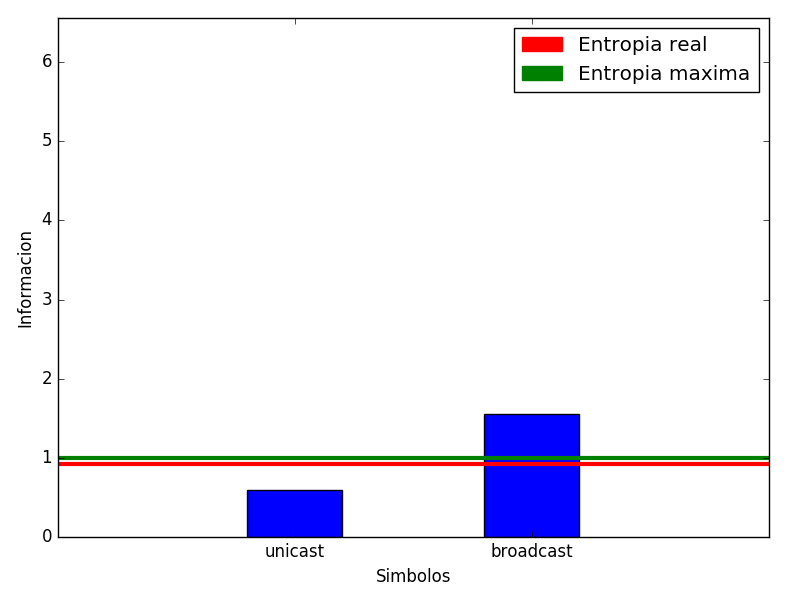
\includegraphics[width=0.7\linewidth]{imagenes/red-dom-S}
\caption{Red doméstica - Fuente S}
\label{fig:red-dom-S}
\end{figure}

Todo este comportamiento se debe a que al haber pocos dispositivos dentro de la red y siempre los mismos, las tablas ARP de cada nodo se mantienen más estables (menos probabilidad de anomalías) y los mensajes broadcast se observan con menos frecuencia.

Fuente S1:

1.93284800528

\begin{figure}[h]
\centering
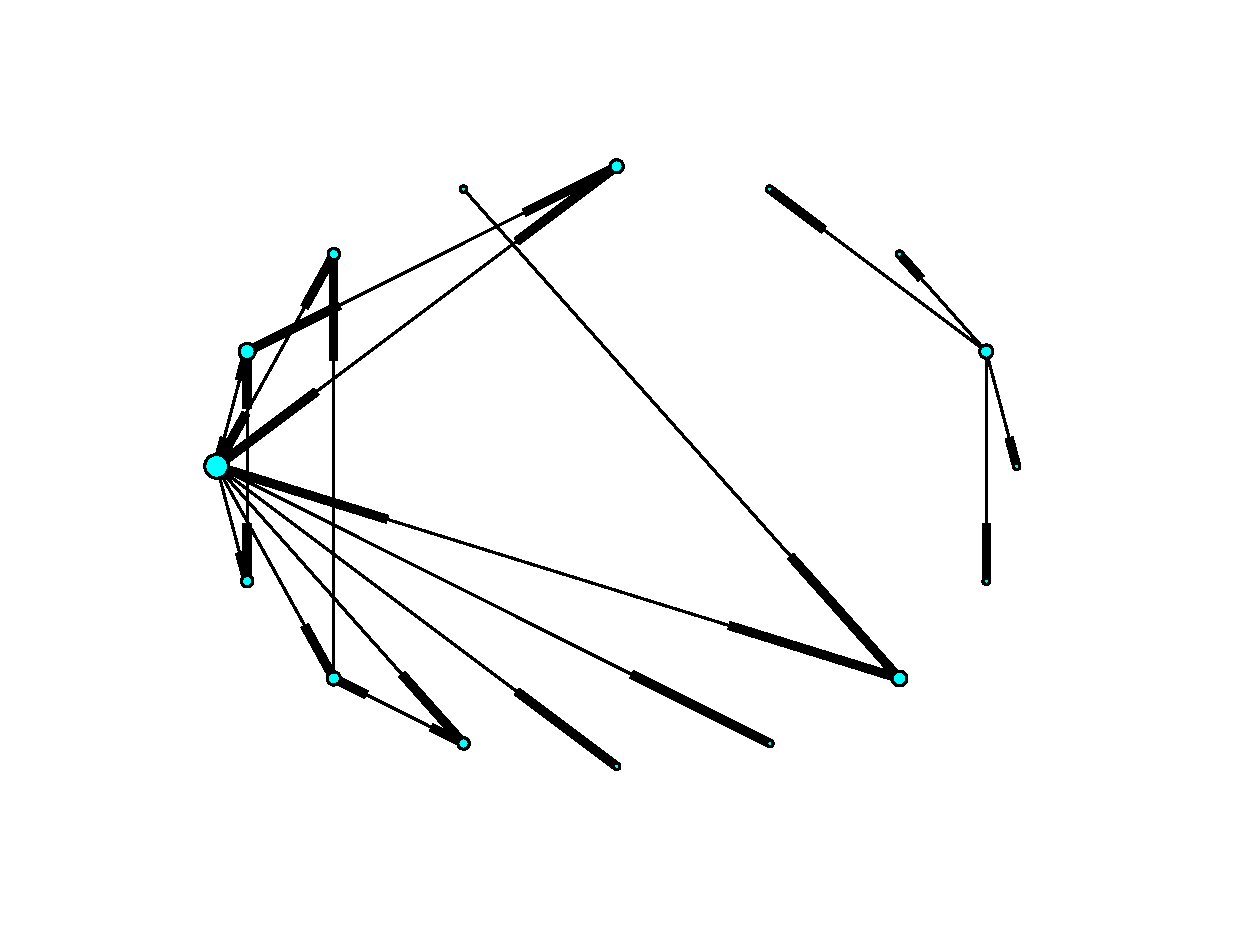
\includegraphics[width=0.7\linewidth]{imagenes/eth-red-domestica}
\caption{}
\label{fig:eth-red-domestica}
\end{figure}

\begin{figure}[h]
\centering
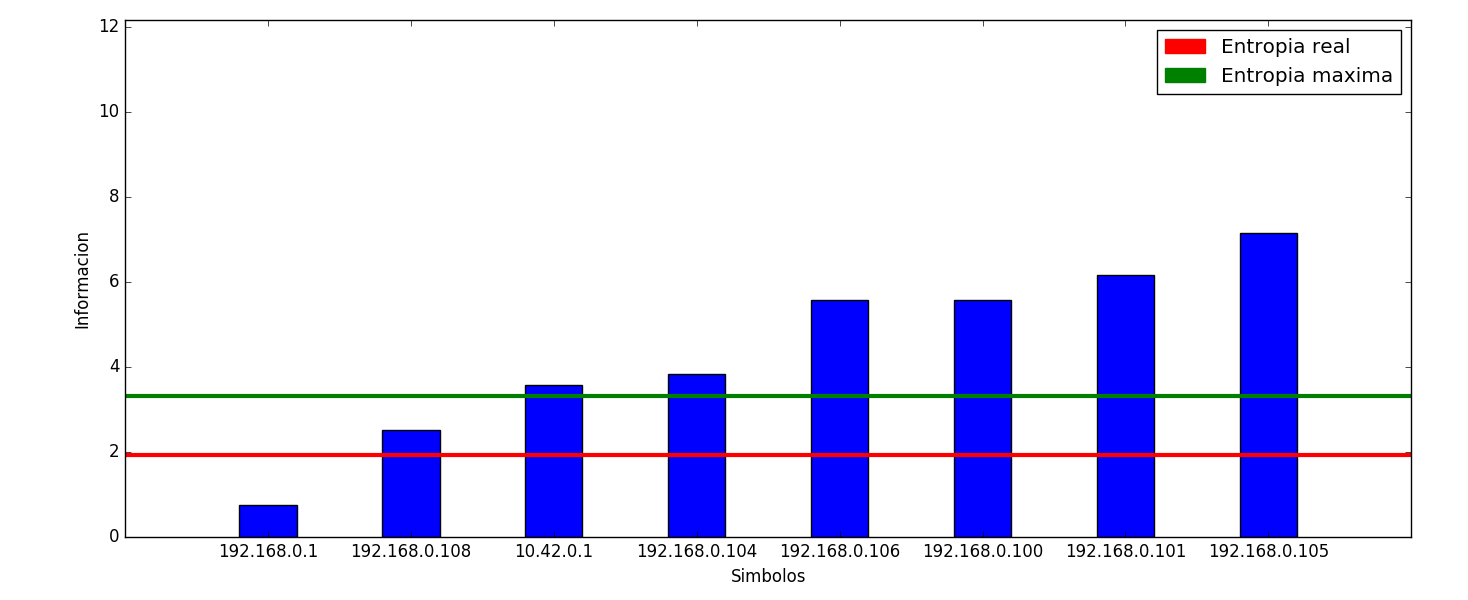
\includegraphics[width=0.7\linewidth]{imagenes/red-dom-S1}
\caption{}
\label{fig:red-dom-S1}
\end{figure}
